\documentclass{simplesnt}

%% Helpful packages
\usepackage{simplebnf}[2023/11/25]
\usepackage{kotex}
\usepackage{xcolor}
\usepackage{amsmath,amssymb}
\usepackage{amsfonts}
\usepackage{tikz}
\usetikzlibrary{calc}
\usepackage{siunitx}
\usepackage{caption}
\usepackage{listings}
\usepackage{mathrsfs}
\usepackage{stmaryrd}
\usepackage{graphicx}

\captionsetup{font=small}
\lstset{basicstyle = \small\ttfamily, breaklines}

\usepackage{tabularray}
\UseTblrLibrary{booktabs}

\usepackage{metalogo}
\usepackage{kotex-logo}


\newcommand{\textalt}[2]{#1\textsubscript{\ensuremath{\text{\scriptsize\textit{#2}}}}}
\newcommand*{\presentfont}[1]{{\fontspec{#1}#1}}
\ExplSyntaxOn
\bool_if:nF { \sys_if_engine_xetex_p: || \sys_if_engine_luatex_p: }
  { \newcommand*{\fontspec}[1]{} }
\ExplSyntaxOff

\title{분석기 골탕 합성 문제 구체화}
\author{정원준}

\begin{document}
\date{2025년 11월 7일}
\maketitle


\begin{frame}
  \frametitle{목차}
  \tableofcontents
\end{frame}

\section{문제 정의}
\begin{frame}[c, fragile]
  \frametitle{간단히 설명하면}

  \begin{columns}[c]
    % 왼쪽: 코드 (고정)
    \begin{column}{0.55\textwidth}
      \lstset{
        language=Python,
        escapeinside={(*@}{@*)},
        basicstyle=\ttfamily\small,
        lineskip=2pt,
        columns=fullflexible,
        aboveskip=6pt,
        belowskip=6pt
      }
\begin{lstlisting}
x = readInt
if (*@\textcolor{red}{x * x - 100 * x + 2500 == 0}:@*)
    x = 0
print x
\end{lstlisting}
    \end{column}

    % 오른쪽: 단계별로 나타나는 텍스트
    \begin{column}{0.4\textwidth}
      \vspace{1em}
      \uncover<2->{\textbf{마지막에서 $x$의 값은?}}

      \bigskip
      \uncover<3->{\textbf{나:} $x \in \mathbb{Z} \setminus \{50\}$}

      \medskip
      \uncover<4->{\textbf{분석기:} $x \in \mathbb{Z}\ (= \top)$}

      \medskip
      \uncover<5->{\textbf{좀 더 좋은 분석기:} $x \in \mathbb{Z} \setminus \{50\}$}
    \end{column}
  \end{columns}

\end{frame}


\begin{frame}
  \uncover<2->{
    \frametitle{Rice 정리}
    \begin{theorem}[Rice's Theorem, Rice 1951]
      $\varphi$를 부분 계산 가능한 함수들의 허용 가능한 \textalt{넘버링}{admissible numbering}이라고 하자.  
      $P \subseteq \mathbb{N}$을 어떤 성질을 만족하는 프로그램들의 인덱스 집합이라고 하자.  
      다음 두 조건을 만족한다고 가정하자:
      \begin{enumerate}
      \item $P$는 \textbf{비자명(non-trivial)}하다. 즉, $P \neq \varnothing$ 이고 $P \neq \mathbb{N}$이다.
      \item $P$는 \textbf{확장적(extensional)}이다. 즉, 모든 $m,n \in \mathbb{N}$에 대해  
      $\varphi_m = \varphi_n$이면 $m \in P \iff n \in P$이다.
      \end{enumerate}
      그렇다면, $P$는 \textbf{결정 불가능(undecidable)}하다.
    \end{theorem}
  }
  
  \vspace{0.3cm}
  \begin{center}
    \uncover<3->{
      \textcolor{red}{``뭐라고요?''}
    }
  \end{center}
\end{frame}

  
\begin{frame}
  \frametitle{우리 상황에 맞게}
이 정리를 우리 문제 상황에 맞게 가공하면 다음과 같다:
  \vspace{0.15cm}
  \uncover<2->{
    \begin{corollary}
      $\mathbb{L}$을 튜링 완전한 프로그래밍 언어라고 하자. 
      $\mathscr{P} \subseteq \mathbb{L}$을 프로그램의 부분집합, 혹은 성질이라 하자. 
      다음 두 조건을 만족한다고 가정하면: 
      
      \begin{enumerate}
      \item $\mathscr{P}$는 \textbf{의미 있는 성질}이다. 즉, $\mathscr{P} \neq \varnothing$ 이고 $\mathscr{P} \neq \mathbb{L}$이다.
      \item $\mathscr{P}$는 \textbf{실행의미에 딱맞는 성질}이다. 즉, $\forall p_1, p_2 \in \mathbb{L}$에 대해  
      $p_1$과 $p_2$의 실행의미가 같으면 $p_1 \in \mathscr{P} \iff p_2 \in \mathscr{P}$이다.
      \end{enumerate}

      다음과 같은 {\scriptsize (항상 유한 시간 안에 끝나는)}분석기 $\mathcal{A}$는 \textbf{존재하지 않는다}:
      $$\forall p \in \mathbb{L}, \mathcal{A}(p) = true \iff p \in \mathscr{P}$$

      다른 말로, \textalt{안전}{sound}하면서 \textalt{완전}{complete}한 분석기를 만들 수 없다.
    \end{corollary}
  }
\end{frame}


\begin{frame}
  \frametitle{공격 목표}
  \textalt{안전}{sound}한 분석기 $\mathcal{A}$를 가정 즉,
  $$\forall p \in \mathbb{L}, \mathcal{A}(p) = true \Rightarrow p \in \mathscr{P}$$
  이다. \uncover<2->{그런데 Rice 정리에 의해
  $$\forall p \in \mathbb{L}, \mathcal{A}(p) = true \iff p \in \mathscr{P}$$
  일 수 없으므로} \uncover<3->{
  $$\forall p \in \mathbb{L}, \mathcal{A}(p) = true \textcolor{red}{\Leftarrow} p \in \mathscr{P}$$
  가 거짓이다.}
\end{frame}

\begin{frame}
  \frametitle{공격 목표}
  $\mathscr{P}$를 ``프로그램 종료 후 변수 x 가 가질 수 있는 값은 $\mathbb{Z}$ 전체가 아니다.''
  로 두면, 다음과 같은 명제를 도출할 수 있다:

  \vspace{0.3cm}
  $\exists p \in \mathbb{L},$
  \vspace{-0.2cm}
  \begin{center}
    $\mathcal{A}(p) = false$ 그리고

    프로그램 종료 후 변수 x 가 가질 수 있는 값은 $\mathbb{Z}$ 전체가 아니다.
  \end{center}
  \uncover<2->{
    이를 만족하는 $p$를 찾는 것이 목표이다.
  }
\end{frame}


\section{가능성}
\begin{frame}
  \frametitle{웬 가능성?}
  평행사변형 \(ABCD\)가 있다. 
  밑변 \(AB\)의 길이가 \(5\)이고 넓이가 \(10\)일 때, 대각선 \(AC\)의 길이는 얼마인가?
  \begin{figure}[h!]
    \centering
    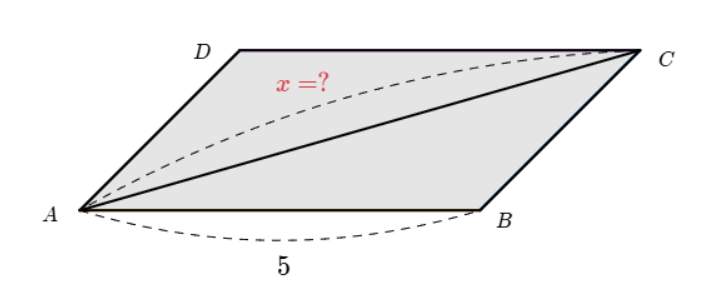
\includegraphics[width=0.7\textwidth]{img/평행사변형.png}
  \end{figure}
\end{frame}


\begin{frame}
  \frametitle{웬 가능성?}
  \vspace{0.5cm}
  반지름의 길이가 1인 원 \(O\)와 O의 한 점을 중심으로 하는 원 \(O'\)가 있다. 
  \(O'\)가 \(O\)의 넓이를 2등분할 때, \(O'\)의 반지름의 길이는 얼마인가?
  \begin{figure}[h!]
    \centering
    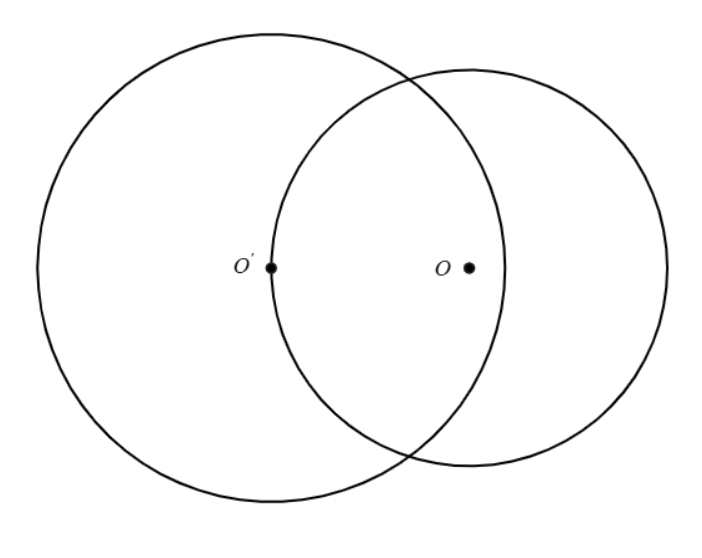
\includegraphics[width=0.5\textwidth]{img/원.png}
  \end{figure}
  \vspace{0.3cm}
  \uncover<2->{
    \begin{center}
      \textcolor{orange}{연구에 대한 정적 분석}
    \end{center}
  }
\end{frame}




\begin{frame}
  \frametitle{전탐색}
  \uncover<1->{recall Rice 정리, 답을 만족하는 프로그램 $p$가 어딘가엔 존재한다.}
  
  \vspace{0.3cm}
  \uncover<2->{그런데 그 $p$를 실제로 유한 시간 안에 찾는 알고리즘이 존재하는지는 모른다.}
  
  \vspace{0.3cm}
  \uncover<3->{프로그램의 개수는 셀 수 있으니까,
  가능한 모든 $p$를 빠짐없이 하나하나 따져나가면 가능하지 않을까?}

  \vspace{0.3cm}
  \uncover<4->{\textcolor{red}{안 됨.} 그렇게 찾은 $i$번째 프로그램 $p_i$가 실제로 $p_i \in \mathscr{P}$인지 알아내는 알고리즘이 없음(다시 Rice정리).}
\end{frame}



\begin{frame}[c, fragile]
  \frametitle{참인 명제 사용}

  처음에 보여줬던 예시: \textcolor{blue}{``$x=50\text{일 때}, (x^2 - 100x + 2500) = 0\text{이다.}$''}
  라는 명제 사용.

  \vspace{0.3cm}
  \uncover<2->{세상에 참인 명제는 셀 수 있이 많은데, 분석기가 그 중 하나쯤은 모르지 않을까?}

  \vspace{0.3cm}
  \uncover<3->{분석기는 공격기를 볼 수 없지만, 분석기는 공격기를 볼 수 있다.}

  \vspace{0.3cm}
  \uncover<4->{힐베르트 프로그램을 흉내 내어, 참인 명제를 순서대로 마구 생성해가면서 분석기에게 이를 시험해 보면 되지 않을까?}

  \vspace{0.3cm}
  \uncover<5->{분석기가 무한히 이어지는 모든 시험에 통과하기는 정말 어려울 것 같다.}

  \vspace{0.3cm}
  \uncover<6->{정말 이렇게 해보겠다는 건 아니고, 만약 이 방법이 정말 어렵지만 성공적이라면, 합성으로 우회해서도 가능하지 않을까?}
\end{frame}



\section{G 언어}
\begin{frame}
  \frametitle{문법}
  \[
    \begin{array}{rcl}
      P & \rightarrow & C \\[1em]
      C & \rightarrow & x := E \\
        & \mid & C ; C \\
        & \mid & \text{ifp } E \; C \; C \\
        & \mid & \text{whilep } E \; C \\[1em]
      E & \rightarrow & n \quad (n \in \mathbb{Z}) \\
        & \mid & x \\
        & \mid & E \text{+} E \\
        & \mid & E \text{*} E \\
        & \mid & \text{-}E
    \end{array}
  \]
\end{frame}

\begin{frame}
  \frametitle{실행의미}
  \textalt{무엇 의미구조}{denotational semantics}로 정의한다.
  \begin{align*}
    Val &= \mathbb{Z} \\
    n &\in Val \\
    M &\in Mem = Var \xrightarrow{\text{fin}} Val \\
    x &\in Var \\
    P, C &\in Cmd \\
    E &\in Exp \\
    \llbracket \cdot \rrbracket_{(C)} &: Cmd \rightarrow Mem \rightarrow Mem \\
    \llbracket \cdot \rrbracket_{(E)} &: Exp \rightarrow Mem \rightarrow Val
  \end{align*}
\end{frame}


\begin{frame}
  \frametitle{실행의미}
  $\llbracket E \rrbracket_{(E)}$의 의미
  \begin{align*}
      \llbracket n \rrbracket M &= n \\
      \llbracket x \rrbracket M &= M(x) \\
      \llbracket E_1 \text{+} E_2 \rrbracket M &= \llbracket E_1 \rrbracket M + \llbracket E_2 \rrbracket M \\
      \llbracket E_1 \text{*} E_2 \rrbracket M &= \llbracket E_1 \rrbracket M \times \llbracket E_2 \rrbracket M \\
      \llbracket \text{-} E \rrbracket M &= - \llbracket E \rrbracket M\\
  \end{align*}
  $\llbracket C \rrbracket_{(C)}$의 의미
  \begin{align*}
      \llbracket x := E \rrbracket M &= M\{x \mapsto \llbracket E \rrbracket M\} \\
      \llbracket C_1 ; C_2 \rrbracket M &= \llbracket C_2 \rrbracket (\llbracket C_1 \rrbracket M)  \\
      \llbracket \text{ifp } E \; C_1 \; C_2 \rrbracket M &= if \; \llbracket E \rrbracket M > 0 \; then \; \llbracket C_1 \rrbracket M \; else \; \llbracket C_2 \rrbracket M \\
      \llbracket \text{whilep } E \; C \rrbracket M &= lfp \; (\lambda f. \lambda M. if \; \llbracket E \rrbracket M > 0 \; then \; f(\llbracket C \rrbracket M) \; else \; M)
  \end{align*}
\end{frame}

\begin{frame}
  \frametitle{참고사항}
  \begin{itemize}
    \item \uncover<2->{G 언어의 문법에는 입/출력이 없다.}
    \vspace{0.3cm}
    \item \uncover<3->{대신 프로그램 전체의 실행의미를 $\llbracket P \rrbracket_{(C)}$로 정의하여
          초기 메모리의 상태를 입력, 나중 메모리의 상태를 출력으로 생각한다.}
    \vspace{0.3cm}
    \item \uncover<4->{non-relational 요약해석으로는 모든 변수가 $\top$인 상태로 시작한다.
          (프로그램이 무한루프에 빠지는지, 도달하지 못하는 라인이 있는지에는 관심 없다)}
  \end{itemize}
\end{frame}



\section{합성 방법}
\begin{frame}
  \frametitle{$\top$이 아님을 어떻게 보장?}
  
  \begin{itemize}
    \item 앞서 언급했듯이, 아무렇게나 $p$를 만들어 놓으면 진짜로 $p \in \mathscr{P}$인지 알기 어려움
    \vspace{0.3cm}
    \item \uncover<2->{따라서 빈 칸이 있는 프로그램에 대해 이미 알고 있는 정보를 들고다니면서 합성해나가야 할 것}
    \vspace{0.3cm}
    \item \uncover<3->{아직 잘 모르겠음}
  \end{itemize}

\end{frame}

\section{마저할일}
\begin{frame}
  \frametitle{마저할일}
  \begin{itemize}
    \item 간단한 분석기 $\mathcal{A}$ 구현하기
    \vspace{0.3cm}
    \item 마구 합성 시도해보기
    \vspace{0.3cm}
    \item 잘 안 될 때마다 왜 안 되는지 명료하게 기록하기
  \end{itemize}
\end{frame}

\definecolor{mydarkblue}{RGB}{32,56,61}

\setbeamercolor{background canvas}{bg=mydarkblue}
\setbeamercolor{normal text}{fg=white}
\setbeamercolor{frametitle}{fg=white}
\addtocounter{framenumber}{-1} % 마지막 슬라이드 번호를 하나 줄임
\appendix
\begin{frame}[c] % [c]는 내용 수직 가운데 정렬
  \centering
  {\Large \textcolor{white}{감사합니다}}
\end{frame}


\end{document}
